% !TeX root = ../thesis.tex

\chapter{Grundlagen}
\label{sec:fundamentals_related-work}

In diesem Kapitel findet zun\"achst eine Einordnung der Trajektorienplanung in das Gesamtsystem von automatisierten Fahrzeugen statt.
Nachdem klar definiert ist was die Aufgabe der Trajektorieplanung ist, werden einige f\"ur die Trajektorienplanung relevante Grundlagen der Optimierung  erl\"autert, sowie Optimierungsverfahren vorgestellt.
Anschlie{ss}end wird ein \"Uberblick \"uber die kooperative Verhaltensplanung gegeben.
Au{\ss}erdem wird das in dieser Arbeit verwendete Frenet"=Koordinatensystem vorgestellt.
Das Kapitel endet mit einem kurzen \"Uberblick zu verwandten Arbeiten der kooperativen Verhaltensplanung.

\section{Einordnung der Trajektorienplanung}
\label{Einordung_Trajktorieplanung}
Die Trajektorienplanung ist neben der maschinellen Wahrnehmung eines der wichtigsten Teilmodule automatisierter Kraftfahrzeuge.
Sie bestimmt das Verhalten des Ego"=Fahrzeuges zum gegenw\"artigen Zeitpunkt und in naher Zukunft.
Dies geschieht basierend auf einem Lagebild der Fahrzeugumgebung, welches in der maschinellen Wahrnehmung generiert wurde. \cite{Ziegler2017}
Als Ego"=Fahrzeug wird in der Literatur h\"aufig das betrachtete Fahrzeug, f\"ur das die Trajektorienplanung stattfindet, bezeichnet.
Diese Bezeichnung wird auch in dieser Arbeit verwendet.

Die Architektur eines autonom fahrenden Fahrzeuges l\"asst sich oftmals in drei Module einteilen: maschinelle Wahrnehmung, Planung und Regelung.  
Die Trajektorienplanung ist dabei der Planung zuzuordnen.  

\begin{figure}[!htbp]
    \centering
    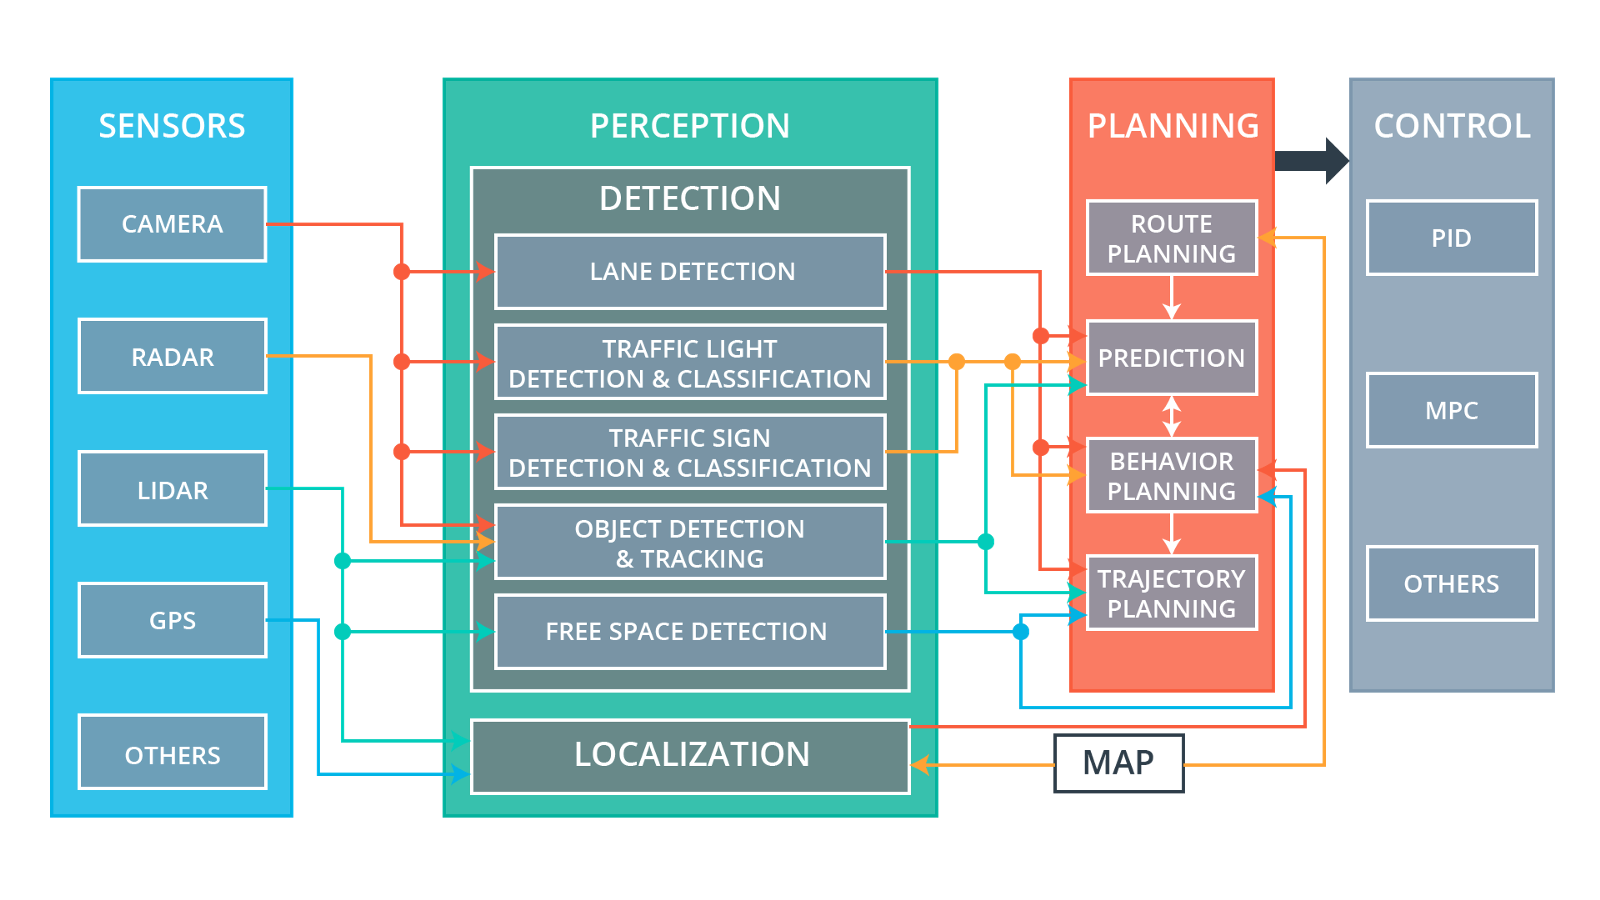
\includegraphics[width = 0.8 \textwidth ]{ADArchtiecture.png}
    \caption[Architektur autonomer Fahrzeuge]{Architektur eines autonomen fahrenden Fahrzeuges \gls{medium}}
    \label{fig:ADArchtiecture}
\end{figure}

F\"ur die maschinelle Wahrnehmung kann entweder ein kartenbasierter Ansatz oder ein rein sensorischer Ansatz genutzt werden.
Bei einem kartenbasierten Ansatz werden Eigenschaften des statischen Verkehrsraums in einer Karte hinterlegt \cite{Ziegler2017}. 
Solche Eigenschaften sind beispielsweise der Verlauf von Fahrstreifen. 
Es k\"onnen ebenfalls Informationen wie Geschwindigkeitsbegrenzungen oder Vorfahrtsregelungen hinterlegt werden. 
Hierdurch sind f\"ur das Fahrverhalten grundlegende Informationen direkt vorhanden und k\"onnen schnell abgerufen werden. 
F\"ur einen kartenbasierten Ansatz wird jedoch ein zus\"atzliches Lokalisationsmodul notwendig.
Aufgabe dieses Lokalisationsmodules ist es, die Position des Fahrzeuges relativ zur Karte zu bestimmen.
Hierzu k\"onnen unter anderem GPS basierte, eigenbewegungsbasierte oder kartenbasierte Positionssch\"atzungen  genutzt werden. 
H\"aufig ergibt sich die Positionssch\"atzung aus einer probabilistischen Kombination der vorher genannten Varianten. 
Diese Informationen m\"ussen bei rein sensorischer Wahrnehmung erst noch generiert werden, was eine hohe Anforderung an das Wahrnehmungsmodul darstellt. 
Die rein sensorische Wahrnehmung hat allerdings den Vorteil, dass keine Lokalisation mehr notwendig ist und dass sie unsensibel gegen\"uber Ver\"anderungen der als statisch angenommen Umgebung ist.
Ein detaillierte Karte mit Fahrstreifenverl\"aufen ist nicht notwendig.
Doch auch bei einem rein sensorischen Ansatz m\"ussen grundlegende Stra{\ss}eninformation hinterlegt sein um die Route des Fahrzeuges planen zu k\"onnen.
In beiden F\"allen muss zus\"atzlich noch eine Wahrnehmung der dynamischen Umgebung stattfinden.
Teil der dynamischen Umgebung sind beispielsweise andere Verkehrsteilnehmer wie Fahrzeuge und Fu{\ss}g\"anger oder aber ein Ampellicht. \cite{Ziegler2017}

Aus den in der Wahrnehmung generierten Daten wird ein Lagebild mit den Informationen zur Fahrzeugumgebung erzeugt \cite{Ziegler2017}. 
Dieses Lagebild wird im Planungsmodul, welches sich dem Wahrnehmungsmodul anschlie{\ss}t, genutzt. 
Neben der Trajektorienplanung k\"onnen auch die Routenplanung, die Pr\"adiktion und die Man\"overplanung zum Planungsmodul gez\"ahlt werden. 
In der Routenplanung wird in einem gegebenen Stra{\ss}ennetz die optimale Route zwischen zwei geographischen Positionen ermittelt \cite{Zhang2013}. 
Diese Aufgabe \"ahnelt der Aufgabe die bei menschlich gef\"uhrten Fahrzeugen heute h\"aufig von einem Navigationssystem \"ubernommen wird. 
In der Pr\"adiktion wird ausgehend vom aktuellen Zustand der Fahrzeuge pr\"adiziert wie sich eine Verkehrssituation in n\"achster Zukunft entwickeln wird.
Dabei werden die zuk\"unftigen Positionen und Zust\"ande der einzelnen Fahrzeuge vorherbestimmt \cite{Hermes2009}.


Die Man\"overplanung bestimmt ein Reihe von auszuf\"uhrenden Man\"overn.
Dies geschieht basierend auf der Fahraufgabe, welche sich aus der Routenplanung ableitet, dem angenommenen Verhalten anderer Verkehrsteilnehmer und der umgebenden Stra{\ss}e.
Ein Man\"over bestimmt das taktische Verhalten eines Fahrzeuges als Reaktion auf die lokale Fahrzeugumgebung. \cite{Zhang2013}
Ein typisches Man\"over ist ein Fahrstreifenwechsel. 
Aufgabe der Trajektorienplanung ist es nun anhand der gegebenen Informationen das Verhalten des eigenen Fahrzeuges in n\"achster Zukunft zu bestimmen \cite{Ziegler2017}. 

H\"aufig ist das Planungsmodul hierarchisch aufgebaut und die einzelnen Elemente besitzen nach unten hin abnehmende Planungshorizonte und Neuplanungsintervalle. 
So kann der Planungshorizont einer Routenplanung mehrere Stunden betragen und es kann eine vergleichsweise lange Zeit zwischen zwei Planungsschritten in Kauf genommen werden. 
Die Trajektorienplanung, als unterstes Glied der Hierarchie besitzt in der Regel einen Planungshorizont im Sekundenbereich und das Neuplanungsintervall kann im Millisekundenbereich liegen. 
Naumann und Stiller \cite{Naumann2017towards} zeigen jedoch, dass es nicht immer sinnvoll ist die einzelnen Planungsschritte getrennt voneinander durchzuf\"uhren.
In der von ihnen vorgestellten Arbeit zur kooperativen Verhaltensplanung wird die Pr\"adiktion und die Man\"overplanung in die Trajektorienplanung integriert.

Aufgabe des Regelungsmoduls, als letztes Glied der Kette ist es, das Fahrzeug entlang der aus dem Planungsmodul erhaltenen Solltrajektorie zu f\"uhren \cite{Ziegler2017}. 
Ein \"Uberblick der Gesamtarchitektur ist in Abbildung~\ref{fig:ADArchtiecture} gegeben.

Auch wenn die Begriffe Pfad und Trajektorie oft synonym verwendet werden soll an dieser Stelle auf deren Unterschied hingewiesen werden.  
So stellt ein Pfad die geometrische Verbindung zwischen einem Startzustand und einem Zielzustand dar. 
Eine zeitliche Komponente wird nicht ber\"ucksichtigt. 
Eine Trajektorie hingegen ber\"ucksichtigt die Zeit. 
Damit sind auch Information wie der Geschwindigkeitsverlauf in einer Trajektorie enthalten und es kann eine Kollisionspr\"ufung mit dynamischen Hindernissen durchgef\"uhrt werden. 
Diese Unterscheidung soll auch im Rahmen dieser Arbeit verwendet werden. \cite{Rathgeber2016}


\section{Optimierungsverfahren in der Trajektorienplanung}
Ziel der Optimierung ist die Ermittlung eines Optimums. 
Dieses Optimum soll in einem wohldefinierten Sinne optimal sein \cite{Ziegler2017}.
So kann mittels eines Navigationssystems die optimale Route im Sinne der geringsten Fahrzeit oder im Sinne des k\"urzesten Weges gesucht werden.
Ziel der Trajektorienplanung ist die Ermittlung einer optimalen Trajektorie \gls{symb:x_optTra} \( = (x(t), y(t))^T \). 
In diesem Kapitel soll zun\"achst eine Formulierung des Optimierungsproblems f\"ur die Trajektorieplanung stattfinden.
Anschlie{\ss}end sollen einige L\"osungsverfahren vorgestellt werden, die bei der Trajektorieplanung zum Einsatz kommen.


\subsection{Formulierung des Optimierungsproblems}
Generell k\"onnen Optimierungsprobleme zwei verschiedenen Gruppen zugeordnet werden. 
Statische Optimierungsprobleme und dynamische Optimierungsprobleme.

\begin{itemize}
\item \textit{Statisches Optimierungsproblem}: Minimierung einer Funktion mit Optimierungsvariablen,
die Elemente des Euklidischen Raumes sind.
\item \textit{Dynamisches Optimierungsproblem}: Minimierung eines Funktionals, bei dem die
Optimierungsvariablen Elemente des Hilbert"=Raumes sind (z.B. Zeitfunktionen). \cite{Graichen2012}
\end{itemize}

Wie in Kapitel \ref{Einordung_Trajktorieplanung} erl\"autert ist eine Trajektorie, im Gegensatz zum Pfad, eine zeitabh\"angige Funktion.
Damit wird deutlich, dass die dynamische Optimierung die f\"ur die Trajektorieplanung relevante Optimierung darstellt. 
Aus diesem Grund soll im Weiteren nur noch die dynamische Optimierung betrachtet werden.

Laut F\"ollinger \cite{Follinger1988} ist, um berechtigterweise von einer Optimierung zu sprechen, ein G\"utema{\ss} notwendig. 
Dieses G\"utema{\ss} ist eine Ma{\ss}zahl, durch welche die Qualit\"at eines Systemverhaltens bewertet wird.
Bei einem Trajektorieplanungsproblem wird damit also die Qualit\"at einer Trajektorie bewertet.
Ziel der Optimierung ist es nun, das G\"utema{\ss} entweder zu minimieren oder zu maximieren. 
Soll das G\"utema{\ss} minimiert werden, so wird das G\"utema{\ss} bei einer dynamischen Optimierung im Allgemeinen als Kostenfunktional bezeichnet.
Soll es maximiert werden, so kann von einem Belohnungsfunktional gesprochen werden.
Ob ein Kostenfunktional oder ein Belohnungsfunktional vorliegt spielt f\"ur die Optimierung kaum eine Rolle, da jedes Belohnungsfunktional in eine Kostenfunktional umgewandelt werden kann \cite{Graichen2012}.
Diese Eigenschaft ist durch das Dualit\"atsprinzip gegeben.
Daher kann im Weiteren von einem Kostenfunktional ausgegangenen werden, das es zu minimieren gilt.
Bei der Verwendung eines Kostenfunktionals ist jede Abweichung von der Optimaltrajektorie mit der Entstehung von Kosten verbunden.

Die zu ermittelnde Optimaltrajektorie soll nicht nur Kollisionsfreiheit garantieren sondern auch komfortabel sein.
Mit dem Ziel den Komfort und die Glattheit der Trajektorie zu steigern wird in der Literatur zur Trajektorienplanung h\"aufig die Geschwindigkeit, die Beschleunigung und der Ruck bei der Optimierung ber\"ucksichtigt \cite{Ziegler2017} \cite{Werling2011}.
Der Ruck ist die Ableitung der Beschleunigung nach der Zeit.
Das Kostenfunktional enth\"alt dann au{\ss}er der Trajektorienfunktion \gls{symb:x_optTra} \(=(x(t), y(t))^T \) auch ihre Ableitungen bis zum dritten Grad.
Damit ergibt sich eine Ruck"=Zeit"=optimale Trajektorie als L\"osung des Optimierungsproblems.
Das G\"utefunktional dieses Optimierungsproblems kann als

\begin{equation} 
  J = \int_{t_0}^{t_e} L( \pmb{x}, \pmb{\dot{x}}, \pmb{\ddot{x}}, \pmb{\dddot{x}}, t) dt
  \label{eq:Kostenfunktional}
\end{equation} 

formuliert werden (vgl. \cite{Ziegler2017}). Dabei stellen \( t_0\) und \( t_e\) den Anfangs- und Endzeitpunkt des Optimierungszeitraums dar.
Bei einer Trajektorienplanung wird dieser Optimierungszeitraums auch als Planungshorizont bezeichnet.

Zus\"atzlich zum Kostenfunktional m\"ussen Randbedingungen und in der Regel auch Nebenbedingungen festgelegt werden, die einzuhalten sind \cite{Follinger1988}.
Die Randbedingungen ergeben sich bei der Trajektorienplanung durch den Start- und  Endzustand des Fahrzeuges.
Vielmals soll in der Trajektorienplanung jedoch kein festdefinierter Endzustand festgelegt werden, da vielmehr ein Zielverhalten von Interesse ist. 
So ist beim Fahren auf einer Stra{\ss}e, \"ahnlich wie bei einem menschlichen Fahrer, weniger von Interesse an welcher Position sich das Fahrzeug am Ende des Planungshorizont befindet. 
Es ist eher von Interesse, dass sich das Fahrzeug noch immer in der Fahrbahnmitte befindet und mit einer Geschwindigkeit  f\"ahrt, die m\"oglichst nahe an der Wunschgeschwindigkeit ist.
Der Endpunkt des Optimierungsproblems ist somit nicht mehr vorgegeben sondern liegt innerhalb von einer Punktemenge des Zustandraumes, einer sogenannten Zielmannigfaltigkeit \(Z\) \cite{Follinger1988}. 

Die Nebenbedingungen ergeben sich aus \"au{\ss}eren und inneren Beschr\"ankungen. 
\"Au{\ss}ere Nebenbedingung betreffen die Umgebung des Fahrzeuges. 
Sie ergeben sich beispielsweise aus Hindernissen oder dem Stra{\ss}enverlauf. 
Dabei geht es immer um Kollisionsfreiheit. 
Die inneren Nebenbedingungen ergeben sich aus Grenzen der Fahrdynamik (zum Beispiel minimale Kurvenradien oder maximale Beschleunigungen) oder aus anderen Beschr\"ankungen wie zum Beispiel der Vorgabe einer maximalen Geschwindigkeit. \cite{Ziegler2017}
Diese Nebenbedingungen schr\"anken den Suchraum ein und k\"onnen entweder als Gleichungsbedingungen

\begin{equation} 
  f( \pmb{x}, \pmb{\dot{x}}, \pmb{\ddot{x}}, \pmb{\dddot{x}}, t) = 0
  \label{eq:Kostenfunktional}
\end{equation} 

oder als Ungleichungsbedingungen

\begin{equation} 
  h( \pmb{x}, \pmb{\dot{x}}, \pmb{\ddot{x}}, \pmb{\dddot{x}}, t) \leq 0
  \label{eq:Kostenfunktional}
\end{equation} 

ber\"ucksichtigt werden \cite{Papageorgiou1991}.
Ungleichungsbedingungen werden in vielen F\"allen ber\"ucksichtigt, indem sie in Gleichungsbedingungen transformiert werden.
Dies geschieht durch die Einf\"uhrung einer Schlupfunktion. \cite{Papageorgiou1991}

Sind das Kostenfunktional sowie Rand- und Nebenbedingungen gegeben, besteht das Optimierungsproblem nun darin, unter allen Trajektorien welche die Rand- und Nebenbedingungen erf\"ullen, diejenige zu finden, welche das Kostenfunktional zum globalen Minimum macht \cite{Follinger1988}.
Hierbei soll auf den Unterscheid zwischen einem globalen und einem lokalen Minimum hingewiesen werden.
Ein globales Minimum beschreibt das Minimum aller Vektoren, welche die Rand- und Nebenbedingungen erf\"ullen. 
Somit ergibt sich f\"ur ein Extremwertproblem, bis auf in sehr wenigen Ausnahmen, nur ein einziges globales Minimum. 
Ein lokales Minimum stellt hingegen nur ein Minimum in einer gewissen Umgebung dar. 
Nur falls es das einzige lokale Minimum ist, ist es auch sicher das globale Minimum. \cite{Follinger1988}


\begin{figure}[!htbp]
    \centering
    \subfigure[Mehrere lokale L\"osungen des Trajektorienplanungsproblems \cite{Ziegler2017}]{
        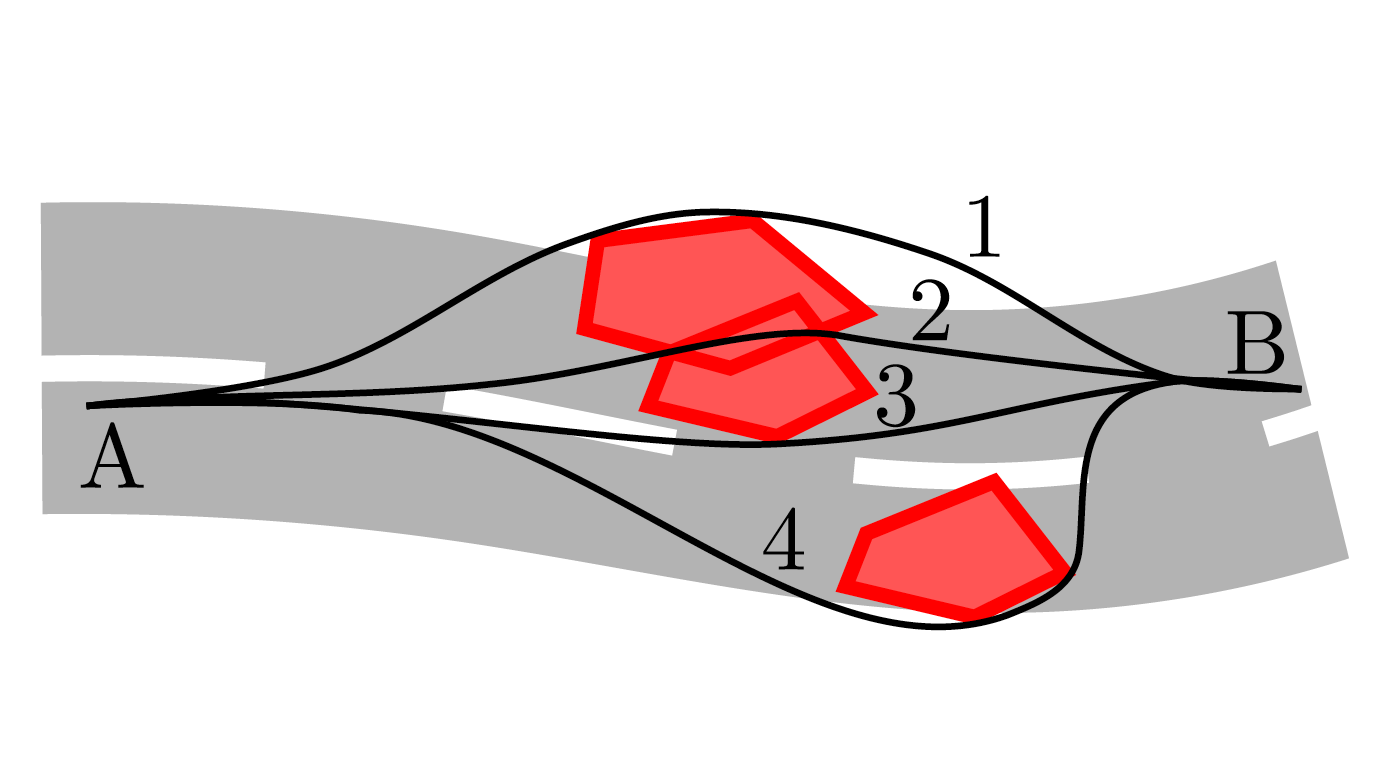
\includegraphics[width = 0.45 \textwidth]{LokalMinimum.png}
        \label{fig:LokalMinimum}
    }
    \hfill
     %add desired spacing between images, e. g. ~, \quad, \qquad, \hfill etc.
     %(or a blank line to force the subfigure onto a new line)
    \subfigure[Globale L\"osung des Trajektorienplanungsproblems \cite{Ziegler2017}]{
        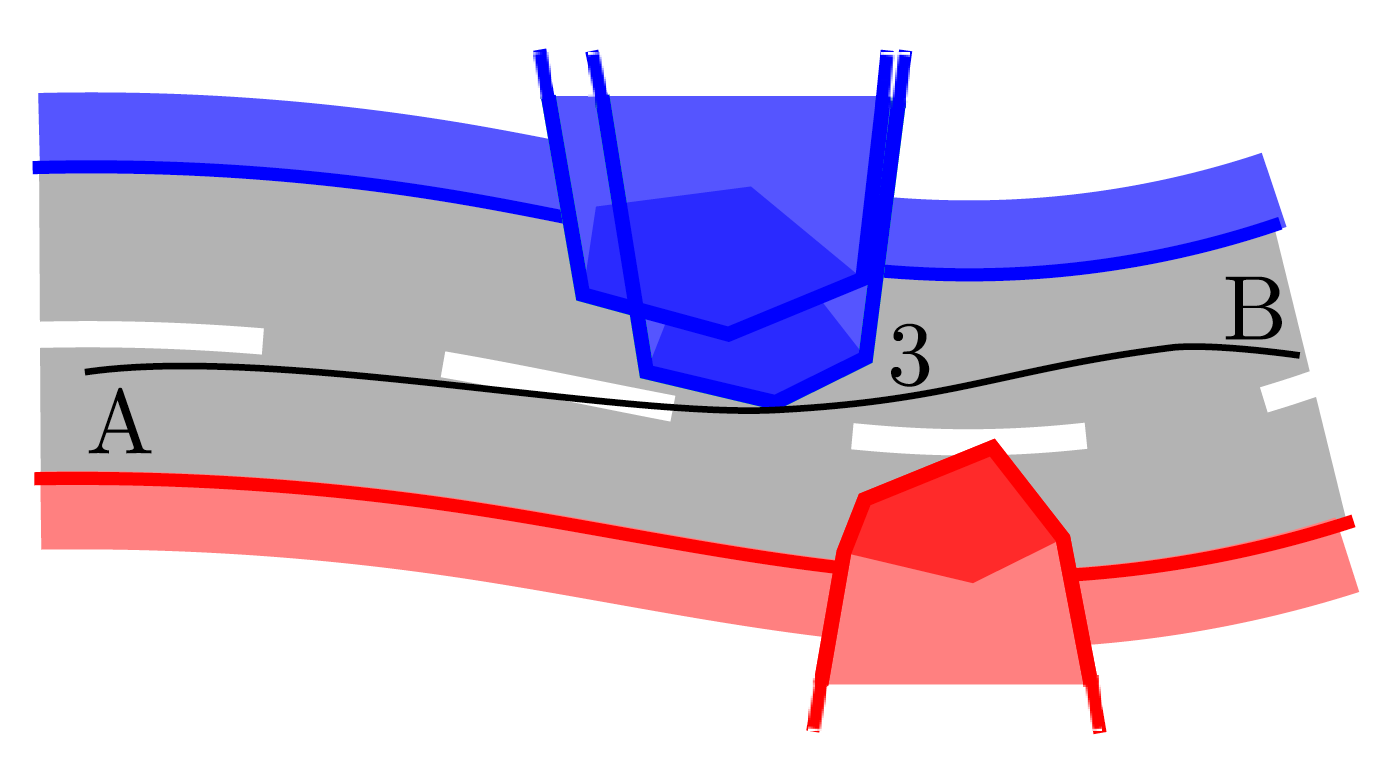
\includegraphics[width = 0.45  \textwidth]{GlobalesMinimum.png}
        \label{fig:GlobalesMinimum}
    }
    \caption[Anpassung f\"ur globales Minimum]{Anpassung des Trajektorienplanungsproblems zur Ermittlung des globalen Minimums}
    \label{fig:GlobalMinAdaption}
\end{figure}


Ziegler \cite{Ziegler2017} zeigt, dass es bedingt durch die Lage von Hindernissen zu mehreren lokalen Minima bei der Trajektorienplanung kommen kann. 
Dies ist in Abbildung~\ref{fig:LokalMinimum} dargestellt.
Nur eines von ihnen entspricht auch dem globalen Minimum.
Das ein gefundenes lokales Minimum das einzige im Suchraum ist und somit auch dem globalen Minimum entspricht kann nur bei konvexen Optimierungsproblemen sichergestellt werden.
Damit sich ein konvexes Optimierungsproblem ergibt, m\"ussen sowohl das Kostenfunktional als auch die Nebenbedingungen konvex sein. 
Ist ein Optimierungsproblem konvex, so k\"onnen im Allgemeinen einfachere und schnellere lokale L\"osungsverfahren genutzt werden. \cite{Graichen2012}
Somit stellt die Konvexit\"at eine wichtige Eigenschaft bei der Auswahl des L\"osungsverfahrens dar. 
Ist die Konvextit\"at nicht gegeben, kann versucht werden das Optimierungsproblem so anzupassen, dass sich ein konvexes Optimierungsproblem ergibt.
Eine Anpassung f\"ur das in Abbildung~\ref{fig:LokalMinimum} dargestellte Trajektorienplanungsproblem ist in Abbildung~\ref{fig:GlobalesMinimum} zu sehen.
Hier werden die Hindernisse jeweils einem Stra{\ss}enrand zugeordnet und die Polygone entsprechend nach au{\ss}en erweitert.
Dadurch f\"uhrt das Optimierungsproblem nur noch zu einem einzigen lokalen Minimum das dadurch auch gleichzeitig dem golbalen Minimum entspricht.

Im Folgenden sollen nun einige L\"osungsverfahren die in der Trajektorienplanung zum Einsatz kommen k\"onnen vorgestellt werden.



\subsection{Variationsrechnung}
\label{sec:Varationsrechnung}
Eine Vielzahl von L\"osungsverfahren beruhen auf der im Ende des 17. und Anfang des 18. Jahrhunderts entwickelten Variationsrechnung. 
Durch sie k\"onnen notwendige Bedingungen f\"ur das gesuchte Minimum abgeleitet werden und dadurch das Optimierungsproblem auf ein Randwertproblem zur\"uckgef\"uhrt werden.
Dies erm\"oglicht eine analytische L\"osung des Optimierungsproblems.
Analytische Verfahren k\"onnen in der Trajektorienplanung nur beschr\"ankt eingesetzt werden, da sie nur in sehr einfachen F\"allen angewendet werden k\"onnen. 
Eine analytische L\"osung ist nur dann m\"oglich, wenn keine expliziten Nebenbedingungen f\"ur Hindernisse, Stellbeschr\"ankungen und an die Fahrdynamik gestellt werden \cite{Ziegler2017}. \cite{Papageorgiou1991}

In vielen F\"allen kann das aus der Variationsrechnung abgeleitete Randwertproblem nur numerisch gel\"ost werden.
Ist dies der Fall wird von einem indirekten numerischen L\"osungsverfahren gesprochen.
Im Vergleich zu direkten numerischen L\"osungsverfahren, bei denen nicht das Randwertproblem sondern das Optimierungsproblem an sich numerisch gel\"ost wird, ist die Initialisierung schwieriger und die Ber\"ucksichtigung von Nebenbedingungen umst\"andlich \cite{Papageorgiou1991}. 
Allerdings ergeben Verfahren, die auf der Variationsrechnung beruhen hochgenaue L\"osungen und dadurch generiertes Wissen kann in der Trajektorienplanung genutzt werden.
So finden variationsrechnungsbasierte Ans\"atze in den Verfahren zur Trajektoriengenierung von Werling \cite{Werling2011} und Rathgeber \cite{Rathgeber2016} Anwendung. \cite{Papageorgiou1991}

F\"ur ein Minimum des Kostenfunktionals

\begin{equation} 
  J = \int_{t_0}^{t_e} L( x, \dot{x}, \ddot{x}, \dddot{x}, t) dt
  \label{eq:Kostenfunktional2}
\end{equation} 

mit der Funktion \(x(t)\), ergibt sich durch die Variationsrechnung folgende Differentialgleichung:

\begin{equation} 
  \frac{\delta L}{\delta x} - \frac{d}{dt} \left(\frac{\delta L}{\delta \dot{x}}\right) + \frac{d^2}{dt^2} \left(\frac{\delta L}{\delta \ddot{x}}\right) - \frac{d^3}{dt^3} \left(\frac{\delta L}{\delta \dddot{x}}\right) = 0
  \label{eq:EulerPoisson}
\end{equation} 

(vgl. \cite{Ziegler2017}). 
Sie wird als EULER"=POISSONschen Differenzialgleichung bezeichnet.
Unter Ber\"ucksichtigung der Anfangs- und Endbedingung ergibt die L\"osung dieses Randwertproblems, dass eine Ruck"=Zeit"=optimale Trajektorie durch ein Polynom 5. Ordnung dargestellt wird.
Diese wird sich in dem von Werling \cite{Werling2011} vorgestellten Verfahren zur Trajektorienplanung zu Nutze gemacht.
Hier wird jeweils f\"ur die laterale und die tangentiale Bewegung eine Schar von Polynomen 5. Ordnung generiert.
Dies geschieht zun\"achst getrennt von einander und ungeachtet von Nebenbedingungen. 
Zur Generierung der Polynomschar wird der Anfangszustand mit unterschiedlichen Endzust\"anden und Endzeitpunkten kombiniert. 
Im Anschluss werden die einzelnen L\"osungen der lateralen und tangentialen Bewegung miteinander kombiniert und auf Einhaltung der Nebenbedingungen untersucht. 
Die Kombination, welche die geringsten Kosten verursacht ergibt die angen\"aherte L\"osung des Optimierungsproblems.



\subsection{Direkte numerische Verfahren}
Bei direkten numerischen Verfahren wird das urspr\"ungliche dynamische Optimierungsproblem in ein statisches Optimierungsproblem umgewandelt. 
Dieses wird dann mittels numerischer Verfahren gel\"ost.
Gesucht wird nun nicht mehr die Funktion \gls{symb:x_optTra}(t) sondern die Positionen \(\pmb{x}_k, \pmb{x}_{k+1}, ..., \pmb{x}_N \) an diskreten St\"utzpunkten der Trajektorie.
Direkte numerische Verfahren wurden durch Fortschritt in der Speicherkapazit\"at und Prozessorleistung in den letzten Jahren immer popul\"arer. \cite{Papageorgiou1991}

Ein direktes numerisches Verfahren mit einer sehr hohen Genauigkeit ist das Kollokationsverfahren \cite{Papageorgiou1991}.
Es findet in dem von Ziegler \cite{Ziegler2017} vorgestellten lokalen, kontinuierlichen Verfahren zur Trajektorienplanung Anwendung. 
Bei Verfahren dieser Art wird durch eine zeitlich Diskretisierung des Problems der L\"osungsraum durch St\"utzstellen parametrisiert.
Die St\"utzstellen werden dann von der Optimaltrajektorie interpoliert.
F\"ur dieses Vorgehen wird das Integral des Kostenfunktionals durch eine endliche Summe ersetzt. 
Unter Verwendung des Finitdifferenzenverfahrens zur Berechnung der ersten und zweiten Ableitung wird das Kostenfunktional

\begin{equation} 
  J = \int_{t_0}^{t_e} L( x, \dot{x}, \ddot{x} , t) dt
\end{equation} 

durch

\begin{equation} 
  J = \sum_{i=1}^{n-2} L( t_i, x_i, \frac{\delta x_i}{2h}, \frac{\delta^2 x_i}{h^2} , h^2)h
\end{equation} 

ersetzt . Dabei gibt \(n\) die Anzahl der St\"utzpunkt an und \gls{symb:h} die Schrittweite.  \cite{Ziegler2017}
Es kann gezeigt werden, dass die L\"osung des statischen Ersatzproblems bei  \gls{symb:h} \(\to 0\) gegen die exakte L\"osung des Optimierungsproblems konvergiert \cite{Papageorgiou1991}.
In \cite{Ziegler2017} wird das statische Ersatzproblem durch das Verfahren der sequenziellen quadratische Programmierung (SQP) gel\"ost.
Dies ist ein Verfahren, um nichtlineare Optimierungsprobleme unter nichtlinearen Nebenbedingungen zu l\"osen


\subsection{Globale L\"osungsverfahren}
\label{globaleLV}
Beim Fahren in einer hochsturkturierten Umgebung, gegeben durch die Stra{\ss}e, entspricht die lokale L\"osung h\"aufig der globalen L\"osung \cite{Ziegler2017}.
Deshalb sind lokale L\"osungsverfahren in vielen F\"allen ausreichend.
Bei einer kooperativen Trajektorienplanung, die h\"aufig kombinatorische F\"ahigkeiten erfordert, ergeben sich jedoch in der Regel nichtkonvexe Optimierungsprobleme.
Somit muss hier in zumeist auf globale L\"osungsverfahren zur\"uckgegriffen werden, mit denen die L\"osung angen\"ahert wird.

\minisec{Randomisierte Verfahren}
Ein Ansatz zur Ermittlung von globalen L\"osungen bilden randomisierte Verfahren. 
Hierbei werden verschiedene L\"osungskandidaten zuf\"allig oder deterministisch generiert, anhand des Kostenfunktionals bewertet und anschlie{\ss}end der Kandidat mit den geringsten berechneten Kosten ausgew\"ahlt.
Allerdings sind solche L\"osungsverfahren nicht vollst\"andig da sie nicht terminieren, wenn f\"ur ein gegebenes Problem keine L\"osung existiert.
Weiter noch kann Optimalit\"at prinzipiell erst nach unendlich langer Laufzeit garantiert werden \cite{Ziegler2017}.
Da dies nicht m\"oglich ist muss aus rechenzeittechnischen Gr\"unden nach einer bestimmten Anzahl von L\"osungskandidaten oder nach einer bestimmten Zeit abgebrochen werden.
Die L\"osung ist nun der bis dahin beste L\"osungskandidat.
Sie entspricht einer Ann\"aherung an die optimale L\"osung.

Eine M\"oglichkeit die Qualit\"at der Versuch im Verlauf der Berechnung zu verbessern bieten metaheuristische Verfahren.
Damit ist es m\"oglich die exakte L\"osung schneller anzun\"ahern.
Basierend auf den bisher bekannten Informationen wird entschieden, welche L\"osungskandiaten als n\"achstes ausprobiert werden sollen.
Dieses Vorgehen wird als Ausbeutung (englisch: exploration) bezeichnet.
Es birgt jedoch die Gefahr gegen ein lokales Minimum zu konvergieren.
Deshalb muss auf ein gutes Verh\"altnis zwischen Ausbeutung und der Erkundung (englisch: exploitation) neuer Bereiche geachtet werden. \cite{Weise2009}

\minisec{Graphenbasierte Verfahren}
Graphenbasierte Verfahren bieten eine weitere M\"oglichkeit zur Ermittlung von global minimalen L\"osungen.
Sie werden h\"aufig zur Pfadgenerierung in unstrukturierter Umgebung angewandt \cite{Ziegler2017}.
Graphen bieten in der Optimierung eine Datenstruktur zur Modellierung von Optmierungsproblemen. 
Auf diese Datenstruktur kann dann ein Optimierungsverfahren angewandt werden.
Ein Graph ergibt sich aus einer Menge von Knoten und Kanten.
Die Knoten bilden diskrete Zust\"ande des L\"osungsraums ab.
Kanten stellen eine Verbindung zwischen zwei aufeinander folgende Konten dar.
Die Kanten k\"onnen gewichtet werden.
Die Gewichtung stellt die Kosten dar um von einem diskreten Zustand in den n\"achsten zu gelangen. 
Ein Graph mit gewichteten Kanten ist beispielhaft in Abbildung~\ref{fig:Graph} abgebildet.
Die Kantengewichte werden anhand einer Kostenfunktion ermittelt.
Ein Pfad ergibt sich nun aus der Abfolge von Knoten, die mit dem Startknoten beginnt und mit dem Zielknoten endet.
Die Kosten des Pfades ergeben sich aus der Summe der Gewichte aller Kanten die dabei abgefahren werden. \cite{Ziegler2017}
Ziel der Optimierung ist es nun den Pfad zu finden, f\"ur den die Summe der Kantengewichte minimal ist.

Die dynamische Programmierung bietet eine M\"oglichkeit diese L\"osung effizient zu finden.
Sie beruht auf dem Prinzip von Bellman.
Es besagt:

\begin{quote}
    \glqq Die Gesamtstrategie kann nur dann optimal sein, wenn jede Reststrategie optimal ist, ganz gleich, von welchem Zwischenstand. \grqq{}
\end{quote}

Basierend auf dieser Aussage kann das Optimierungsproblem auf einen mehrstufigen Entscheidungsprozess zur\"uckgef\"uhrt werden. 
Dazu wird zur Ermittlung der optimalen L\"osung im k-ten Schritt auf die optimale L\"osung im vorangegangenen Schritt zur\"uckgegriffen und diese als Endst\"uck der L\"osung des k-ten Schrittes verwendet. 
Diese Strategie ist durch die Rekursionsformel von Bellman beschrieben, die sich direkt aus dem Optimalit\"atsprinzip von Bellman ableitet. 
Beruhend auf dieser Formel wurden zahlreiche Suchverfahren entwickelt. 
Zwei der bekanntesten sind die h\"aufig verwendeten Suchalgorithmen Dijkstra und A*. \cite{Follinger1988}

\begin{figure}[!htbp]
    \centering
    \subfigure[Darstellung eines gewichteten Graphens \cite{Grimme2018}]{
        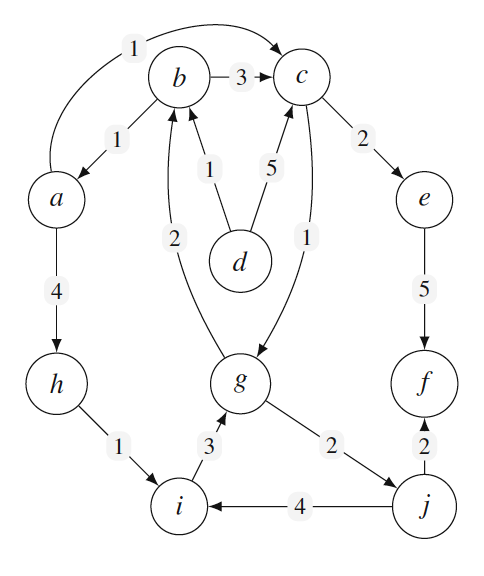
\includegraphics[width = 0.31 \textwidth]{Graph.png}
        \label{fig:Graph}
    }
    \hfill
     %add desired spacing between images, e. g. ~, \quad, \qquad, \hfill etc.
     %(or a blank line to force the subfigure onto a new line)
    \subfigure[Gitter aus Grundgeometrien \cite{Ziegler2009}]{
        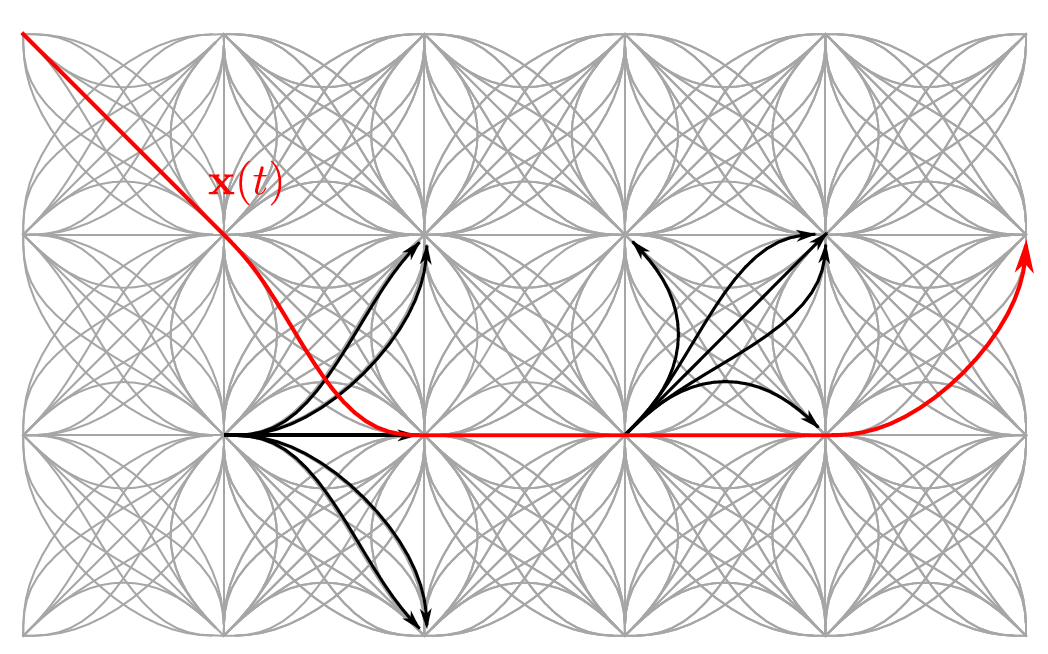
\includegraphics[width = 0.59  \textwidth]{statelatice.png}
        \label{fig:statetlatice}
    }
    \caption[Graphenbasierte Trajektorienplanung]{Graphenbasierte L\"osungsverfahren zur Trajektorienplanung}
    \label{fig:Graphenbasiert}
\end{figure}

Aufgabe der Trajektorienplanung ist es nun die Erstellung eines geeigneten Graphen sowie die Ermittlung der optimalen Trajektorie mittels eines geeigneten Suchalgorithmus.
Der Graph kann basierend auf einer sogenannte Zustandsraumvergitterung (englisch: state lattice) erstellt werden.
Dabei stellen die Gitterpunkte m\"ogliche Zust\"ande des Fahrzeuges dar.
Der Zustand kann zum Beispiel durch die Position und die Orientierung des Fahrzeuges, sowie die Kr\"ummung der Trajektorie beschrieben werden.
Die einzelnen Gitterpunkte werden dann durch einige wenige optimale Grundgeometrien verbunden. 
Die Grundgeometrien sind das Ergebnis eines lokalen Trajektorienplanungsproblems.
Sie ber\"ucksichtigen die inneren Nebenbedingungen und sorgen somit daf\"ur, dass die gefundene Trajektorie fahrbar ist.
Die optimale Trajektorie ergibt sich nun aus einer Kombination der Grundgeometrien.
Sie wird mit Verfahren der dynamischen Programmierung ermittelt. 
Ein solches Gitter aus Grundgeometrien sowie eine zusammengesetzte Beispieltrajektorie (in rot abgebildet) sind in Abbildung~\ref{fig:statetlatice} dargestellt.  \cite{Ziegler2009}



\section{Kooperative Verhaltensplanung}
Laut \cite{Naumann2017towards} und \cite{Lenz2016} ist es wichtig, dass automatisierte Fahrzeuge ein menschen\"ahnliches Fahrverhalten zeigen. 
Daf\"ur gibt es verschiedene Gr\"unde. 
Auf der einen Seite ist ein menschen\"ahnliches Verhalten wichtig, damit nicht automatisierten Fahrzeugen die Pr\"adiktion der automatisierten Fahrzeuge erm\"oglicht bzw. erleichtert wird. 
Auf der anderen Seite ist eine komfortables und menschen\"ahnliches Verhalten wichtig um die Akzeptanz von automatisierten Fahrzeugen zu steigern \cite{Naumann2017towards}. 

Eine essentielle Eigenschaft menschlicher Fahrer ist, dass die Absichten anderer Verkehrsteilnehmer prognostiziert werden und dass diese Absichten dann in der eigenen Verhaltensplanung Ber\"ucksichtigung finden. 
Ein solches Verhalten kann als kooperatives Verhalten gewertet werden. \cite{Lenz2016} 
Situationen in den menschliche Fahrer h\"aufig kooperatives Verhalten zeigen, kommen im realen Verkehr regelm\"a{\ss}ig vor. 
Ulbrich et al. \cite{Ulbrich2015} geben eine knappe \"Ubersicht solcher Situationen. 
Ein h\"aufig vorkommendes Beispiel, in denen menschliche Fahrer \"ublicherweise kooperatives Verhalten zeigen, ist das Auffahren auf die Autobahn. 
Hier kann oft beobachtet werden, dass Fahrzeuge ihre Geschwindigkeit anpassen um Fahrzeugen auf der Beschleunigungsspur das Auffahren zu erleichtern.

Ein solches kooperatives Verhalten ist in manchen Verkehrssituationen nicht nur erstrebenswert sondern sogar eine Voraussetzung f\"ur die erfolgreiche Meisterung der Situation \cite{Lenz2016}. 
Es wird offensichtlich, dass daher ein kooperatives Verhalten auch in der Trajektorienplanung von hochautomatisierten Fahrzeugen ber\"ucksichtigt werden sollte. 
Die meisten bisher bekannten Verfahren zur Trajektorienplanung zeigen jedoch lediglich ein reaktives Verhalten.
Dabei werden andere Verkehrsteilnehmer als bewegte Hindernisse betrachtet.
Der Einfluss des Verhaltens des Ego"=Fahrzeuges auf andere Verkehrsteilnehmer wird zumeist missachtet.
Sind kombinatorische F\"ahigkeiten gefragt, geraten solche Verfahren meist an ihre Grenzen.
Aus diesem Grund sind kooperative Ans\"atze zur Verhaltensplanung von hochautomatisierten Fahrzeugen vermehrt ins Forschungsinteresse ger\"uckt. \cite{Naumann2017towards}

Um ein kooperatives Verhalten in der Trajektorienplanung zu ber\"ucksichtigen ist es zun\"achst einmal wichtig zu betrachten, was ein kooperatives Verhalten ausmacht und wie dieses definiert werden kann. 
In der Literatur sind zahlreiche Definition f\"ur kooperatives Verhalten zu finden. 
So beschreiben Cao et al. \cite{Cao1997}, dass ein System mit mehreren Robotern ein kooperatives Verhalten aufweist, wenn \glqq ein zugrundeliegender Mechanismus f\"ur eine Erh\"ohung des Gesamtnutzen sorgt\grqq{}. 
Doran et al. \cite{Doran1997} beschreiben, dass Kooperieren bedeutet, dass \glqq mit anderen zusammen gehandelt wird um einen gemeinsamen Zweck oder einen gemeinsamen Vorteil zu erreichen\grqq{}. 
In psychologischer Betrachtung kann die Kooperation als eine Form der sozialen Zusammenarbeit zwischen Personen, Gruppen oder Institutionen gesehen werden \cite{Spiess2014}.

In den Ver\"offentlichungen von Naumann et al. \cite{Naumann2017} und Ulbrich et al. \cite{Ulbrich2015} findet jeweils eine Einteilung von kooperativem Verhalten statt. 
Naumann et al. stellen zur Einteilung des kooperativen Verhaltens ein Stufenmodell bestehend aus 5 Stufen vor, wobei von Stufe zu Stufe der Kooperationsgrad gesteigert wird. 
Die Klassifizierung findet anhand der Kenntnisse eines Agenten \"uber den Gesamtnutzen statt. 
Diese Einteilung ist in Tabelle~\ref{tab:koopStufenmodell} gegeben.

\begin{table}
  \centering
  \begin{tabular}{l p{5cm} p{8cm}}
  \hline
  Stufe& Klassifizierung 					& Kenntnis des Gesamtnutzens \\
  \hline
  0   	& unkooperatives Verhalten           		& keine Kenntnis des Gesamtnutzens \\
  1 	& reaktives Verhalten                      		& Kenntnis des Faktors Unfallfreiheit \\
  2 	& vorausschauendes Verhalten 		& Kenntnis einzelner Handlungsoptionen je Verkehrsteilnehmer \\
  3     	& bewusst kooperatives Verhalten 		& Kenntnis mehrerer Handlungsoptionen und deren wechselseitige Abh\"angigkeit je Verkehrsteilnehmer  \\
  4 	& ganzheitlich kooperatives Verhalten	& Kenntnis der m\"oglichen Handlungsoptionen aller relevanten Verkehrsteilnehmer und deren teilnehmer\"ubergreifende wechselseitige Abh\"angigkeit \\
  \hline
  \end{tabular}
  \caption[Kooperatives Stufenmodell]{Stufenmodell zur Einteilung von kooperativen Verhalten \cite{Naumann2017}}
  \label{tab:koopStufenmodell}
\end{table}

In \cite{Ulbrich2015} werden anhand einer Matrix mehreren m\"oglichen Kommunikationskan\"alen die f\"ur eine kooperatives Verhalten genutzt werden k\"onnen, verschiedene Level von kooperativen F\"ahigkeiten gegen\"uber gestellt. Die entsprechende Matrix ist in Abbildung~\ref{fig:coopMatrice} dargestellt.
Es wird ersichtlich, dass eine sogenannte Fahrzeug"=zu"=Fahrzeug"=Kommunikation, bei der explizite Kommunikationskan\"ale genutzt werden um Informationen und auch Intentionen zwischen zwei Fahrzeugen auszutauschen, nur einer der m\"oglichen Kommunikationskan\"ale ist. 
Eine solche Kommunikation war bereits h\"aufig Gegenstand von Untersuchungen, da sie ein hohes Potential an Komfort-, Effizienz-, und Sicherheitssteigerung verspricht. 
Allerdings werden sich automatisierte Fahrzeuge in absehbarer Zeit die Stra{\ss}e vor allem mit menschlich gef\"uhrten Fahrzeugen teilen, die nicht \"uber ein solches Kommunikationssystem verf\"ugen.
Andere Kommunikationsk\"anale wie zum Beispiel gewollte und ungewollte Gesten stellen hohe Anforderungen an die maschinelle Wahrnehmung, die heutige Wahrnehmungsysteme h\"aufig noch nicht erf\"ullen. 
Ein M\"oglichkeit ist jedoch, die Intension andere Fahrkehrsteilnehmer durch ihr Fahrverhalten zu pr\"adizieren und anhand dieser Informationen eine kooperative Trajektorienplanung zu realisieren. \cite{Ulbrich2015}

\begin{figure}[!htbp]
    \centering
    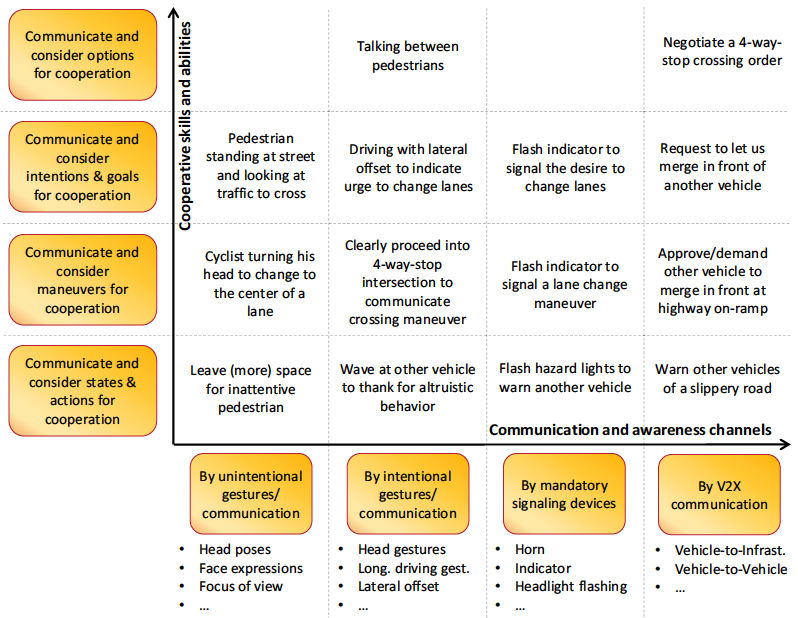
\includegraphics[width = \textwidth ]{KooperationsMatrix.png}
    \caption[Kooperationsmatrix]{Klassifizierung von kooperativer Verhaltensplanung anhand m\"oglicher Kommunikationskan\"ale und notwendigen F\"ahigkeiten \cite{Ulbrich2015}}
    \label{fig:coopMatrice}
\end{figure}




\FloatBarrier


\section{Frenet Koordinatensystem}
\label{sec:Frenet}
Zur Beschreibung der Fahrzeugbewegung stehen verschiedene Koordinatensysteme zur Verf\"ugung. 
G\"angige Koordinatensysteme die in der Bewegungsplanung genutzt werden sind das weltfeste Koordinatensystem, das fahrzeugfeste Koordinatensystem und das Stra{\ss}enkoordinatensystem. 
Abbildung~\ref{fig:FrenetKoord} gibt eine \"Ubersicht \"uber die verschiedenen Koordinatensysteme.
Die Wahl des Koordinatensystems kann starke Auswirkungen auf die Komplexit\"at und somit auch auf die Laufzeit eines Planungsalgorithmus haben. 
Somit spielt die Wahl eines geeigneten Koordinatensystems eine wichtige Rolle in der Trajektorienplanung.
Im Folgenden soll nun das Frenet"=Koordinatensystem vorgestellt werden und seine Nutzung f\"ur die Trajektorienplanung dieser Arbeit motiviert werden.
Eine Beschreibung in Frenet"=Koordinaten entspricht der mathematischen Beschreibung des Stra{\ss}enkoordinatensystems. \cite{Rathgeber2016}

Eine entscheidende Eigenschaft die sich durch die Wahl des Frenet"=Koordinatensystems ergibt ist, dass nicht in Weltkoordinaten geplant wird, sondern entlang einer Referenzkurve.
H\"aufig ist nicht die globale Position des Fahrzeuges relevant, sondern die Position des Fahrzeuges relativ zur Fahrspur und zu anderen Verkehrsteilnehmern \cite{Rathgeber2016}.
Beim Fahren auf einer Stra{\ss}e kann entweder die Fahrbahnmitte oder der linke oder rechte Fahrbahnrand als Referenzkurve gew\"ahlt werden. 
Im Falle einer unstrukturierten Umgebung, beispielsweise beim Fahren auf einer Parkfl\"ache, ist die Referenzkurve das Ergebnis einer Pfadsuche.  \cite{Werling2011}

\begin{figure}[!htbp]
    \centering
    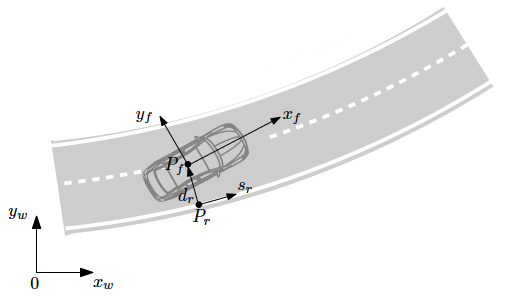
\includegraphics[width = 0.8 \textwidth]{FrenetKoordinaten.png}
    \caption[Koordinatensysteme]{\"Ubersicht \"uber die verwendeten Koordinatensysteme. Dargestellt ist das weltfeste Koordinatensystem (\(F_w = \{0, x_w, y_w\}\)), das fahrzeugfeste Koordinatensystem (\(F_f = \{P_f, x_f, y_f\}\)) und das Stra{\ss}enkoordinatensystem beschrieben in Frenet"=Koordinaten (\(F_r = \{P_r, s_r, d_r\}\)). \cite{Rathgeber2016}}
    \label{fig:FrenetKoord}
\end{figure}

Die Fahrzeugposition wird nun durch die Bogenl\"ange \gls{symb:s_r} entlang der Referenzkurve und den Abstand \gls{symb:d_r} zur Referenzkurve beschrieben. 
Dabei zeigt \gls{symb:s_r} in Richtung des Tangentenvektors \(t({s_r})\) und \gls{symb:d_r} zeigt in Richtung des Normalenvektors \(n({s_r})\).
Der Tangenetenvektor \(t({s_r})\) ist immer tangential zur Referenzkurve ausgerichtet. 
Der Normalenvektor \(n({s_r})\) steht senkrecht zu \(t({s_r})\) und zeigt auf den Referenzpunkt \({P_f}\) des Fahrzeuges. \cite{Rathgeber2016}

Im Planungsmodul wird nun nicht die Bewegung in Richtung \(x_f\) geplant, welche die Richtung entlang der geplanten Trajektorie darstellt.
Stattdessen wird die Bewegung des Fu{\ss}punktes \(P_r\) entlang der Referenzkurve geplant. 
Dadurch ist es m\"oglich die sich ergebende Trajektorie geschlossen zu berechnen. \cite{Werling2011}

Nicht nur die Fahrzeugeigenbewegung, sondern auch alle anderen relevanten Verkehrsteilnehmer werden in Frenet"=Koordinaten betrachtet.
Die Transformation vom Welt- ins Frenet"=Koordinatensystem entspricht anschaulich einer Entkr\"ummung der Fahrbahn \cite{Rathgeber2016}. 
Dies ist in Abbildung~\ref{fig:Fahrbahnentkruemmung} dargestellt. 
Durch die entkr\"ummte Betrachtung der Verkehrssituation ergeben sich einige Vorteile. 
Es vereinfacht sich die Planung f\"ur die Vorgabe von Haltepunkten, sowie von Soll- und Sicherheitsabst\"anden \cite{Werling2011}. 
Au{\ss}erdem kann eine getrennte Optimierung der L\"angs- und Querbewegung des Fahrzeuges \cite{Rathgeber2016} stattfinden. 
Werling \cite{Werling2011} beschreibt des Weiteren, dass sich Vorteile bei der Planung eines Fahrstreifenwechsels auf einer gekr\"ummten Fahrbahn ergeben.
Demzufolge ergibt sich durch die Wahl des Frenet"=Koordinatensystem ein Fahrstreifenwechsel, der mehr einem menschlichen Fahrverhalten \"ahnelt.
Dadurch kann die Bewegung des Fahrzeuges von anderen Verkehrsteilnehmern leichter eingesch\"atzt werden.

\begin{figure}[!htbp]
    \centering
    \subfigure[Verkehrsituation auf gekr\"ummter Fahrbahn \cite{Rathgeber2016}]{
        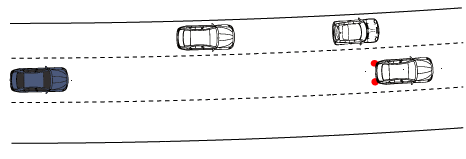
\includegraphics[width = 0.45 \textwidth ]{GekreummtFahrsituation.png}
        \label{fig:lGekruemmteFahrbahn}
    }
    \hfill
     %add desired spacing between images, e. g. ~, \quad, \qquad, \hfill etc.
     %(or a blank line to force the subfigure onto a new line)
    \subfigure[Entkr\"ummte Verkehrssituation \cite{Rathgeber2016}]{
        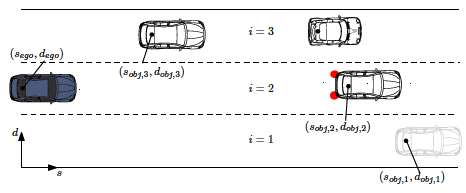
\includegraphics[width = 0.45 \textwidth ]{EntkreummtFahrsituation.png}
        \label{fig:EntkruemmteFahrbahn}
    }
    \caption[Fahrbahnentkr\"ummung]{Visualisierung der Entkr\"ummung der Verkehrssituation durch die Verwendung von Frenet"=Koordinaten}
    \label{fig:Fahrbahnentkruemmung}
\end{figure}

Die Formeln zur Umwandlung von Welt- in Frenet"=Koordinaten und umgekehrt sowie zur Berechnung der Bewegung entlang der Referenzkurve sind in \cite{Werling2011} und \cite{Rathgeber2016} gegeben.




\section{Verwandte Arbeiten}
F\"ur die kooperative Bewegungsplanung automatisierter Fahrzeuge existieren in der Forschung bereits einige Ans\"atze.
In vielen F\"allen wird ein kooperatives Verhalten erreicht indem im Kostenfunktional der Fahrzeuge auch die Kosten andere Verkehrsteilnehmer ber\"ucksichtigt werden.
An dieser Stelle werden nun zwei dieser Ans\"atze exemplarisch vorgestellt.


\subsection{Rekursive Konfliktl\"osung}
In \cite{Schwarting2014} wird ein Planungsalgorithmus f\"ur eine kooperative Verhaltensplanung in einer autobahn\"ahnlichen Umgebung vorgestellt. 
Dieser beruht auf  einer rekursiven Konfliktl\"osung.
F\"ur jedes in Betracht gezogenen Fahrzeug einzeln, beginnend mit dem am weitesten vorne fahrenden Fahrzeug, wird zun\"achst eine egoistische Planung durchgef\"uhrt. 
Basierend auf dieser egoistischen Planung werden dann Konflikte, die durch Interaktion mit anderen Fahrzeugen auftreten detektiert und anschlie{\ss}end \"uber einen Konfliktl\"osungsalgorithmus gel\"ost. 
Die Man\"over, die den Fahrzeugen zur Verf\"ugung stehen, werden durch sogenannte Bewegungsprimitive beschr\"ankt. 
Ein Bewegungsprimitiv wird dabei vollst\"andig beschrieben durch
\begin{itemize}
\item eine Beschleunigungskurve (beschleunige, halte Geschwindigkeit, bremse),
\item einen Bewegungstyp (Fahrstreifenwechsel auf die linke oder rechte Fahrstreifen Fahrstreifen beibehalten),
\item die Bewegungsdauer und
\item den Zeitpunkt der Initiierung.
\end{itemize}
Anstatt einer unendlichen Menge von M\"oglichkeiten stehen den Fahrzeugen somit nur wenige aber zweckm\"a{\ss}ige Man\"over zur Verf\"ugung. 
In Abbildung~\ref{fig:Motionprimit} ist ein Man\"oversatz f\"ur ein Fahrzeug in einer autobahn\"ahnlichen Situation dargestellt.

\begin{figure}[!htbp]
    \centering
    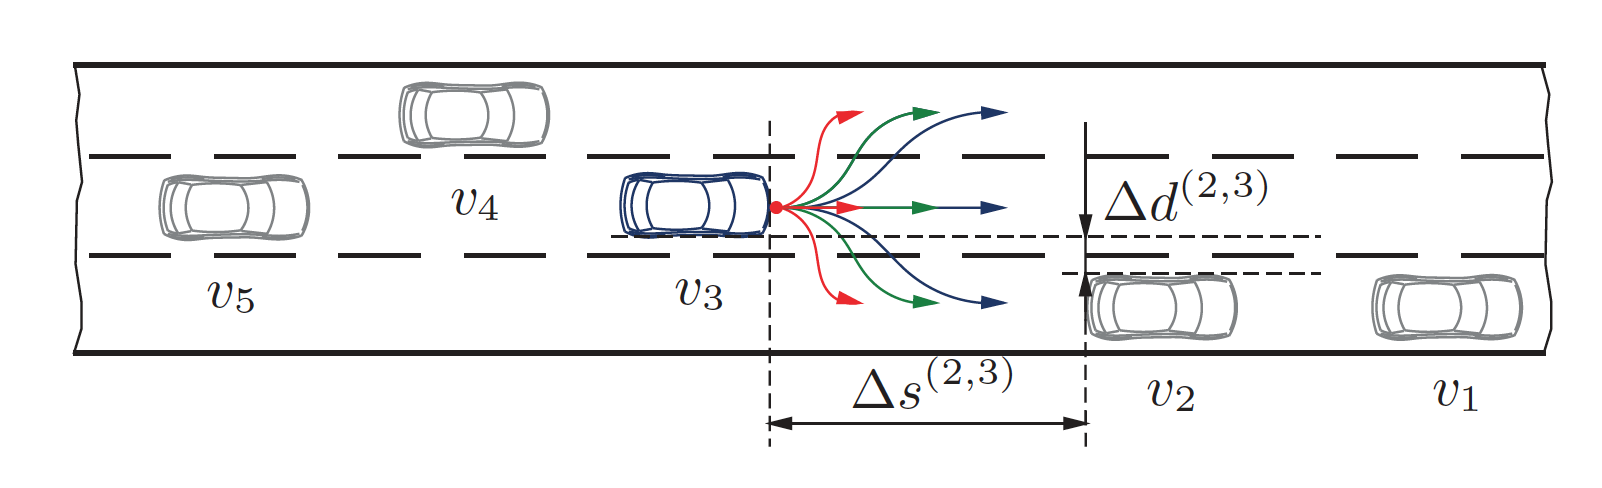
\includegraphics[width = 0.8 \textwidth ]{Motionprimit.png}
    \caption[Bewegungsprimitive]{Satz von m\"oglichen Man\"overn}
    \label{fig:Motionprimit}
\end{figure}

In der egoistischen Planung findet zun\"achst eine Planung statt in der die Interessen anderer Fahrzeuge missachtet werden. 
Endet der Fahrstreifen eines Fahrzeuges wird ein Zeitpunkt \(TTA_{LaneEnd}\) bestimmt, bei dem ein Fahrstreifenwechsel eingeleitet wird. 
Befindet sich vor dem zu betrachtenden Fahrzeug ein langsameres Fahrzeug auf der gleichen Fahrstreifen, wird ein Zeitpunkt \(TTA_{smart}\) bestimmt. 
Dieser Zeitpunkt gibt an, wann ein Fahrstreifenwechsel zum \"Uberholen eingeleitet werden soll. 
Zur Bestimmung von \(TTA_{smart}\) wird sowohl der Abstand, die Differenzbeschleunigung  und die Differenzgeschwindigkeit der Fahrzeuge in Betracht gezogen als auch die Wunschgeschwindigkeit des betrachteten Fahrzeuges.

Nachdem f\"ur alle Fahrzeuge die egoistische Bewegungsplanung durchgef\"uhrt wurde, kommt der rekursive Konfliktl\"osungsalgorithmus zum Einsatz. 
Daf\"ur wird, beginnend mit dem vordersten Fahrzeug, eine Konflikterkennung ausgef\"uhrt in der gepr\"uft wird, ob es durch die egoistische Planung zur Unterschreitung von Sicherheitsabst\"anden kommt. 
Dabei werden nur vorausfahrende Fahrzeuge in Betracht gezogen. 
Falls ein Konflikt detektiert wird, wird eine Konfliktl\"osung ermittelt. 
Daf\"ur werden alle m\"oglichen Man\"overkombinationen der beteiligten Fahrzeuge anhand einer Kostenfunktion bewertet. 
Anschlie{\ss}end wird die Man\"overkombination ausgew\"ahlt, welche die geringsten gemeinsamen Kosten der beiden Fahrzeuge verursacht. 
Dadurch wird ein kooperatives Verhalten aller Fahrzeuge abgebildet.

Wenn alle Fahrzeuge den Konfliktl\"osungsalgorithmus durchlaufen haben ist der Planungsschritt abgeschlossen. 
Die Gesamtl\"osung enth\"alt auch die L\"osung des Ego"=Fahrzeuges. 
Da das Ergebnis stark diskretisiert ist, wird vorgeschlagen dieses an einen Trajektorienplaner weiterzugeben.
Basierend auf dem diskertisierten Ergbnis soll dieser eine komfortable Trajektorie ermitteln.
Hierf\"ur kann der von Werling \cite{Werling2010} vorgestellte ruckminimierende Trajektoriengenerator genutzt werden.

Der Algorithmus wurde sowohl in einer Simulation als auch auf der Autobahn getestet. 
Den Autoren zufolge war der Algorithmus in der Lage Konflikte mit anderen Fahrzeugen zu antizipieren und zu l\"osen.
Es konnten dadurch sinnvolle Fahrman\"over erzeuget werden.

\subsection{Kooperative Planung mit Monte Carlo Tree Search}
Lenz et al. \cite{Lenz2016} stellen einen kombinatorischen Bewegungsalgorithmus basierend auf dem \gls{mcts} vor. 
Ein Baum ist in der Graphentheorie ein spezieller Typ von Graph \cite{Grimme2018}. 
Deshalb kann der vorgestellte Bewegungsalgorithmus zu den Graphen basierten Verfahren gez\"ahlt werden. 
Beim \gls{mcts} handelt es sich um eine randomisierte Suchmethode, welche die Pr\"azision einer Baumsuche mit der Allgemeing\"ultigkeit eines Samplingverfahrenes kombiniert \cite{Browne2012}. 
Der Basisalgorithmus kann in die vier Schritte: Selektion, Expansion, Simulation und R\"uckpropagierung eingeteilt werden. 
Die vier Schritte des Basisalgorithmus sind in Abbildung~\ref{fig:MCTS} visualisiert.

Dieser Basisalgorithmus wird abge\"andert, um ihn auf das Problem der kombinatorischen Bewegungsplanung anzupassen.  
Dazu wird die Planung zeitlich diskretisiert. 
Die in der Planung ber\"ucksichtigten Fahrzeuge k\"onnen Aktionen nur an den diskreten Zeitpunkten ausf\"uhren und tun dies alle simultan. 
Die Planung findet damit in Etappen statt. 
Au{\ss}erdem werden die in Betracht gezogenen Fahrzeuge in interagierende und beeinflusste Fahrzeuge unterteilt.
Die Unterteilung der Fahrzeuge hat Auswirkungen darauf, wie die Fahrzeuge im Planungsalgorithmus behandelt werden.
In Abbildungn~\ref{fig:Klassifizierung} ist die Einteilung der Fahrzeuge f\"ur ein autobahn\"ahnliches Scenario dargestellt.
Im Folgenden sollen nun kurz die einzelnen Schritte des angepassten Algorithmus erl\"autert werden.

\begin{figure}[!htbp]
    \centering
    \subfigure[Die vier Schritte des \gls{mcts} \cite{Browne2012}]{
        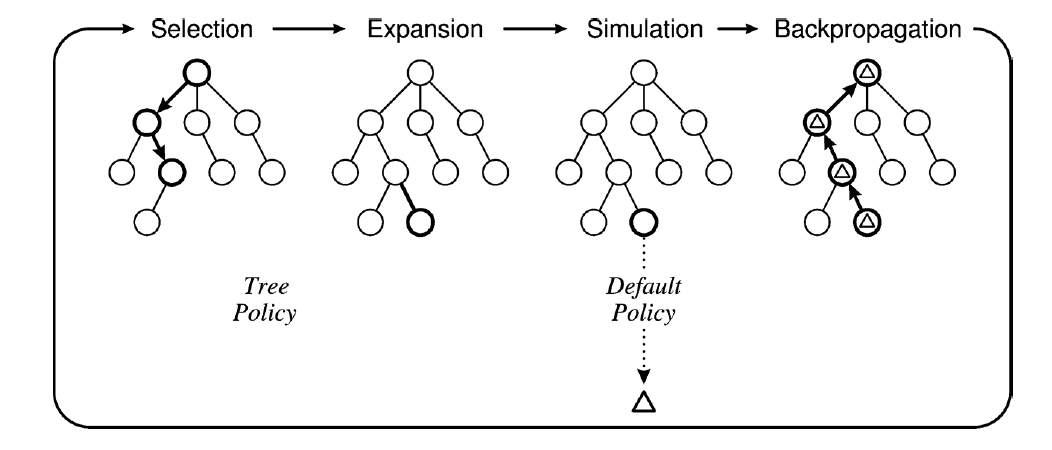
\includegraphics[width = 0.4 \textwidth ]{MCTS.png}
        \label{fig:MCTS}
    }
    \hfill
     %add desired spacing between images, e. g. ~, \quad, \qquad, \hfill etc.
     %(or a blank line to force the subfigure onto a new line)
    \subfigure[Klassifizierung der Fahrzeug (rot: Ego"=Fahrzeug, blau: interagierende Fahrzeuge, wei{\ss}: beeinflusste Fahrzeuge) \cite{Lenz2016}]{
        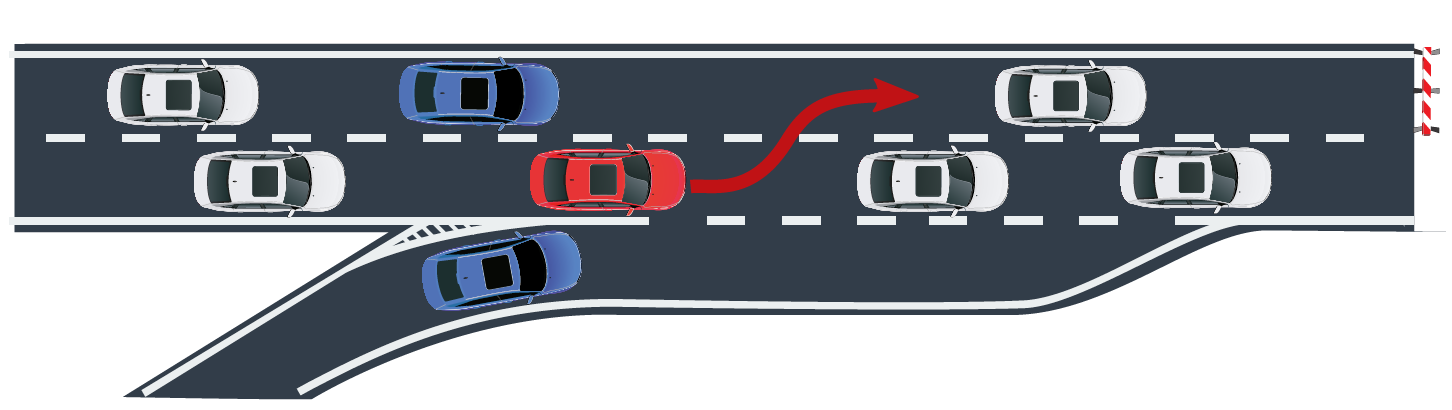
\includegraphics[width = 0.5 \textwidth]{Klassifizierung.png}
        \label{fig:Klassifizierung}
    }
    \caption[Monte Carlo Tree Search]{Kooperative Planung mit dem Monte Carlo Tree Search}
    \label{fig:koopMCTS}
\end{figure}


Im ersten Schritt, dem Selektionsschritt, wird ermittelt welcher Knoten als n\"achstes expandiert werden soll. 
Entsprechend eines gew\"ahlten Auswahlverfahrens wird der Baum nach unten durchlaufen, bis ein Endknoten (Blattknoten) erreicht wurde. 
Hier wurde auf einen gebr\"auchlichen Auswahlalgorithmus zur\"uckgegriffen.

Im Expansionsschritt werden dem nun Baum neue Knoten hinzugef\"ugt. 
Um die simultane Entscheidung der Fahrzeuge in einem Baum darstellen zu k\"onnen werden die Entscheidungen der Fahrzeuge zwar aufeinanderfolgend getroffen, aber bis zum R\"uckpropagierungsschritt verborgen. 
Interagierenden Fahrzeugen steht f\"ur die Entscheidung eine fest vordefinierte Menge von m\"oglichen Aktionen zur Verf\"ugung.
Beeinflusste Fahrzeuge verhalten sich entsprechend dem von Treiber et al. \cite{Treiber2000} vorgestellten \gls{idm}. 
Auf diese wird in Kapitel~\ref{sec:IDMpred} genauer eingegangen. 

Im Simulationsschritt wird nun ausgehend von den neuen Knoten eine Simulation durchgef\"uhrt, die den Ausgang pr\"adizieren soll. 
Als Standartverhalten der Fahrzeuge wird hier erneut das \gls{idm} verwendet. 
Die Kosten der neuen Knoten werden anhand der Kostenfunktion des jeweiligen Fahrzeuges bewertet.
In dieser werden neben Kosten die durch das Verhalten des eigenen Fahrzeuges bedingt sind \"uber einen Kooperationsfaktor auch die Kosten der anderen Fahrzeuge ber\"ucksichtigt. 
Somit wird davon ausgegangen, dass sich alle Fahrzeuge kooperativ verhalten.
Im letzten Schritt, dem R\"uckpropagierungsschritt, werden anhand des Simulationsergebnisses die Statistiken der Knoten entlang des gew\"ahlten Pfades aktualisiert.

Die vier beschriebenen Schritte werden solange wiederholt, bis der Algorithmus abgebrochen wird.
Dadurch werden immer mehr Knoten zum Baum hinzzugef\"ugt und somit immer mehr kombinatorische Bewegungsm\"oglichkeiten untersucht.

Die Autoren heben hervor, dass sich durch die Verwendung des \gls{mcts} mehrere Vorteile ergeben.
Dazu geh\"oren, dass der Algorithmus stark parallelisierbar ist und dass er jederzeit abgebrochen werden kann und ein valides Ergebnis zur\"uckgeben wird.
Der Algorithmus wurde simulativ in Fahrstreifenwechselszenarien verschiedener Komplexit\"at getestet. 
Es konnte gezeigt werden, dass der Algorithmus in der Lage ist ein menschen\"ahnliches kooperatives Fahrverhalten abzubilden.
Es wird au{\ss}erdem beschrieben, dass sich der Algorithmus selbst dann als robust herausgestellt hat, wenn die Kostenfunktion anderer Fahrzeuge falsch eingesch\"atzt wurde oder diese sich suboptimal verhalten.


